\section{Conventional \gls{abb:nas}}\label{sec:hw-nas:nas}

    To address the challenges associated with manual \gls{abb:nn} design highlighted in the chapter's introduction, a new way of designing neural network architectures has emerged : Neural Architecture Search. It is a set of techniques to automatically design neural network architectures. Formulated as an optimization problem, it searches for the best architecture among a set of candidates by maximizing the objective of interest, for example, the accuracy~\cite{NAS-survey}
    
    As most optimization problems, \gls{abb:nas} has 3 important components: the Search Space, Search Strategy and the Evaluation method. In this section, a detailed description of each component is given.

    \subsection{Search Space}

        A search space is a set of candidate neural architectures. It can be designed on three different levels: layer level, cell level and network level. An explanation and an example for each level will be provided followingly.

        \subsubsection{Layer level}
        
        \subsubsection{Cell level}

            A neural network comprises numerous cells, also referred to as building blocks. In this type of \gls{abb:nas} search space design, the goal is to identify one or more performant cell architectures. Subsequentially, we can repeat them $N$ times and connect them to construct a neural network architecture.

            In Figure , we can see that NASNet searches for two cell architectures: a normal cell that preserves the dimensionality of the input, and a reduction cell that reduces the spatial dimension.

             To construct a cell, NASNet represents it as a computation graph that has placeholders for two input hidden states, an operation to apply to each of the two hidden states, and an aggregation operation to combine the results of the two operations, resulting in a new hidden state.
            
            These placeholders are filled by an \gls{abb:rnn} controller that emits several choices at each time stamp. It first selects two hidden states from the previous layer or the layer before that, then it chooses two input transformation operations such as convolution, pooling, or identity, and finally, it selects a method to combine the results, e.g., addition or concatenation. The process is represented in Figure

            Although blocks designed by \gls{abb:nas} provide good accuracy, they are quite complex when compared to manually designed ones. This complexity arises from the intricate dependencies between their elements, making it extremely challenging to map to hardware for efficient inference. For instance, a buffer won't be able to be released until all dependencies are finished computing, necessitating much more memory than is actually needed.


        \subsubsection{Network level}

        When we possess the cells or building blocks for our neural network, the next step is their integration. Such search spaces encompass one or more dimensions for linking these cells. Some of these dimensions include:
        
            • \textbf{Depth:} represents how many times to repeat the building cells. For example, a block might undergo repetition 2, 3, 4 times, and so forth ~\cite{onceforall}.
            
            • \textbf{Resolution:} defines the input dimensions, for example : $(3,128,128)$ , $(3,256,256)$, ... ~\cite{onceforall}
            
            • \textbf{Width:} specifies the number of output channels, i.e. the number of filters to apply.~\cite{onceforall}
            
            • \textbf{kernel size:} determines the dimensions of the convolution filters to apply.~\cite{proxylessnas}

    \subsection{Search Strategy}

        The search strategy defines how to explore the search space, which is often very large or even unbounded. Among the most used algorithms, we find :

        \subsubsection{Grid Search}
            The search search space is a cartesian product of single dimension design spaces. To get the accuracy, a sample is taken from each grid to be trained to get its accuracy.
            

        %\subsubsection{Random Search}

        \subsubsection{Reinforcement Learning}
            To use reinforcement learning  for search space exploration, we model the architecture design as a sequential decision making problem. Reinforcement learning is used to train the \gls{abb:rnn} controller that chooses the neural network elements. The gradient of the probability p is calculated because other components are not differentiable.~\cite{nasrl}

            \textbf{Drawback :} the training is very slow, which drastically increases the search time.

        \subsubsection{Gradient Descent}
            In this type of continuous relaxation to enable direct gradient-based optimization. The output at each node is represented as a weighted sum of outputs from different edges.~\cite{darts}

        \subsubsection{Evolutionary Algorithm}
            In \gls{abb:nas} with evolutionary algorithms, a population of architecture candidates is explored by random sampling within the design space. A fitness function evaluates candidates based on metrics like MACs, number of model parameters, and accuracy. The better candidates are combined and tweaked using evolutionary operations to create a new set of candidates. The process iterates by selecting the best candidates, applying evolutionary operations, adding good resulting candidates to the population and reiterating until an optimal neural network architecture is found. The process can be visualized in~\Cref{fig:hw-nas:nas:evolutionary}

            \begin{figure}[hbt!]
                \begin{center}
                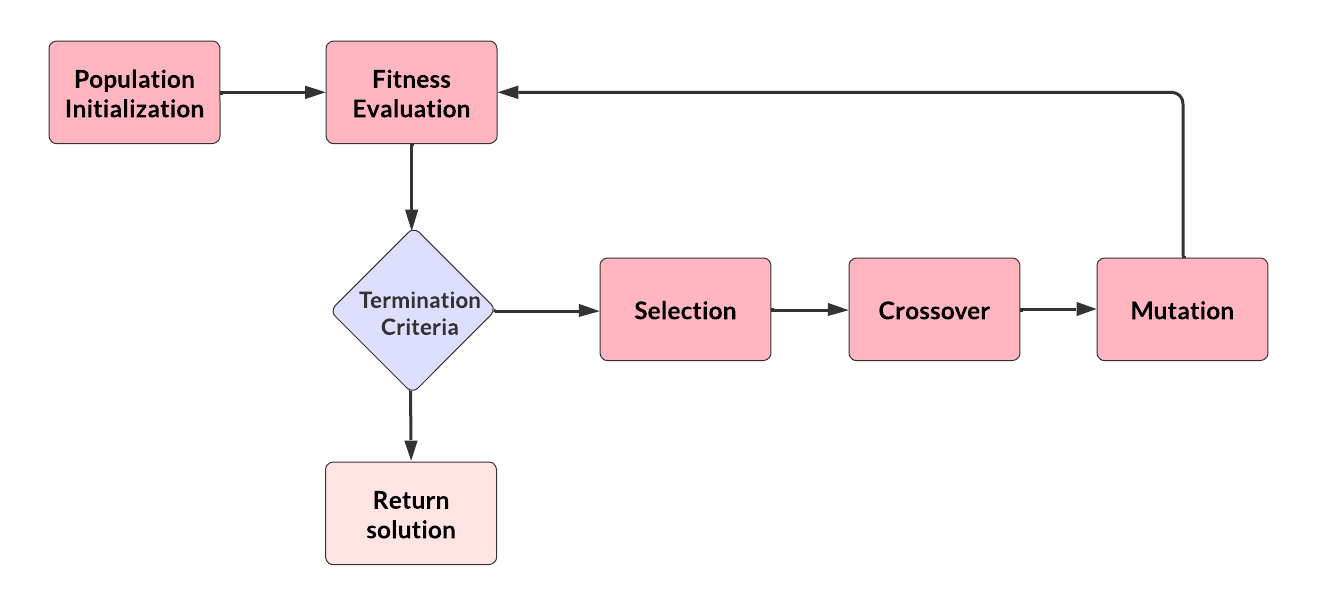
\includegraphics[width=.9\textwidth]{assets/images/evolutionary.png}
                \end{center}
                \caption{Evolutionary Algorithm}%
                \label{fig:hw-nas:nas:evolutionary}
            \end{figure}

            Evolutionary operations are operators that combine and modify candidates to get new ones that are potentially better in terms of  fitness. The most used ones are Mutation and Crossover.
    
                - \textbf{Mutation :}
                
                    Mutation introduces small changes in the candidate architecture to explore novel possibilities. These alterations can be applied on various levels, such as the depth level, as depicted in~\Cref{fig:hw-nas:nas:mudepth}, or on the operator level, as illustrated in~\Cref{fig:hw-nas:nas:mutop}~\cite{onceforall}.

                    \begin{figure}[hbt!]
                        \begin{center}
                        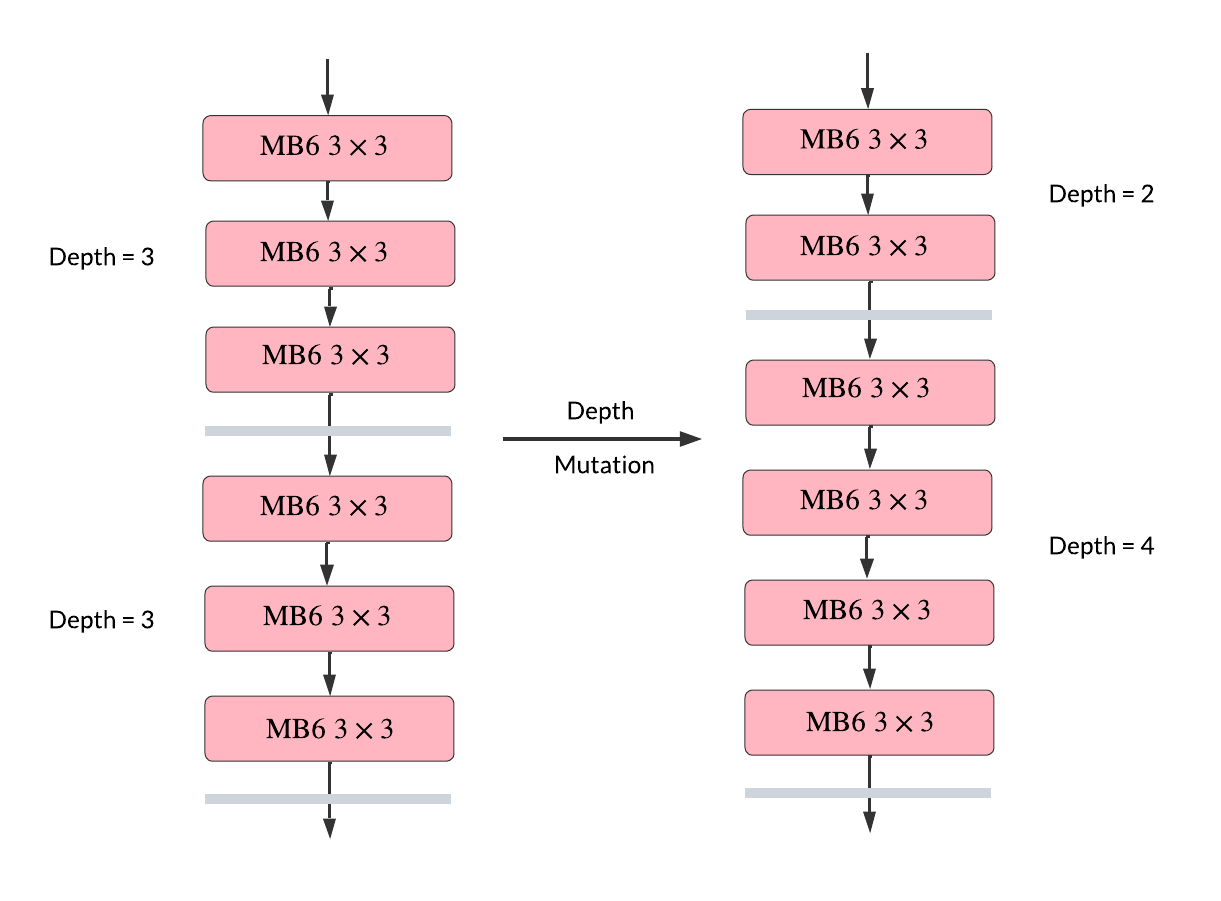
\includegraphics[width=.6\textwidth]{assets/images/mutdepth.png}
                        \end{center}
                        \caption{Mutation on depth}%
                        \label{fig:hw-nas:nas:mudepth}
                    \end{figure}

                    \begin{figure}[hbt!]
                        \begin{center}
                        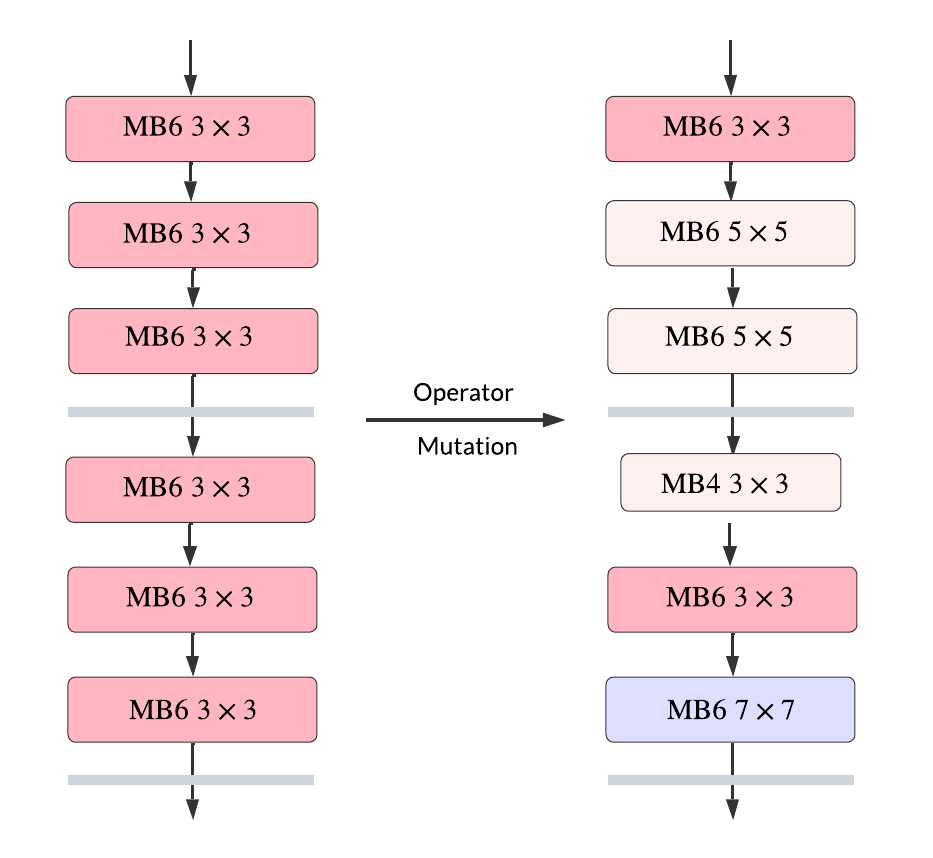
\includegraphics[width=.6\textwidth]{assets/images/mutop.png}
                        \end{center}
                        \caption{Mutation on operator}%
                        \label{fig:hw-nas:nas:mutop}
                    \end{figure}
                    

                - \textbf{Crossover :}
                
                Crossover is an operator that merges parts from high-performing architectures to generate new candidates. It can be done on the operator level to construct a new candidate by, for each layer, randomly selecting one operator an operator from either of two parent architectures~\cite{onceforall}, as dictated in~\Cref{fig:hw-nas:nas:crossover}.

                \begin{figure}[hbt!]
                        \begin{center}
                        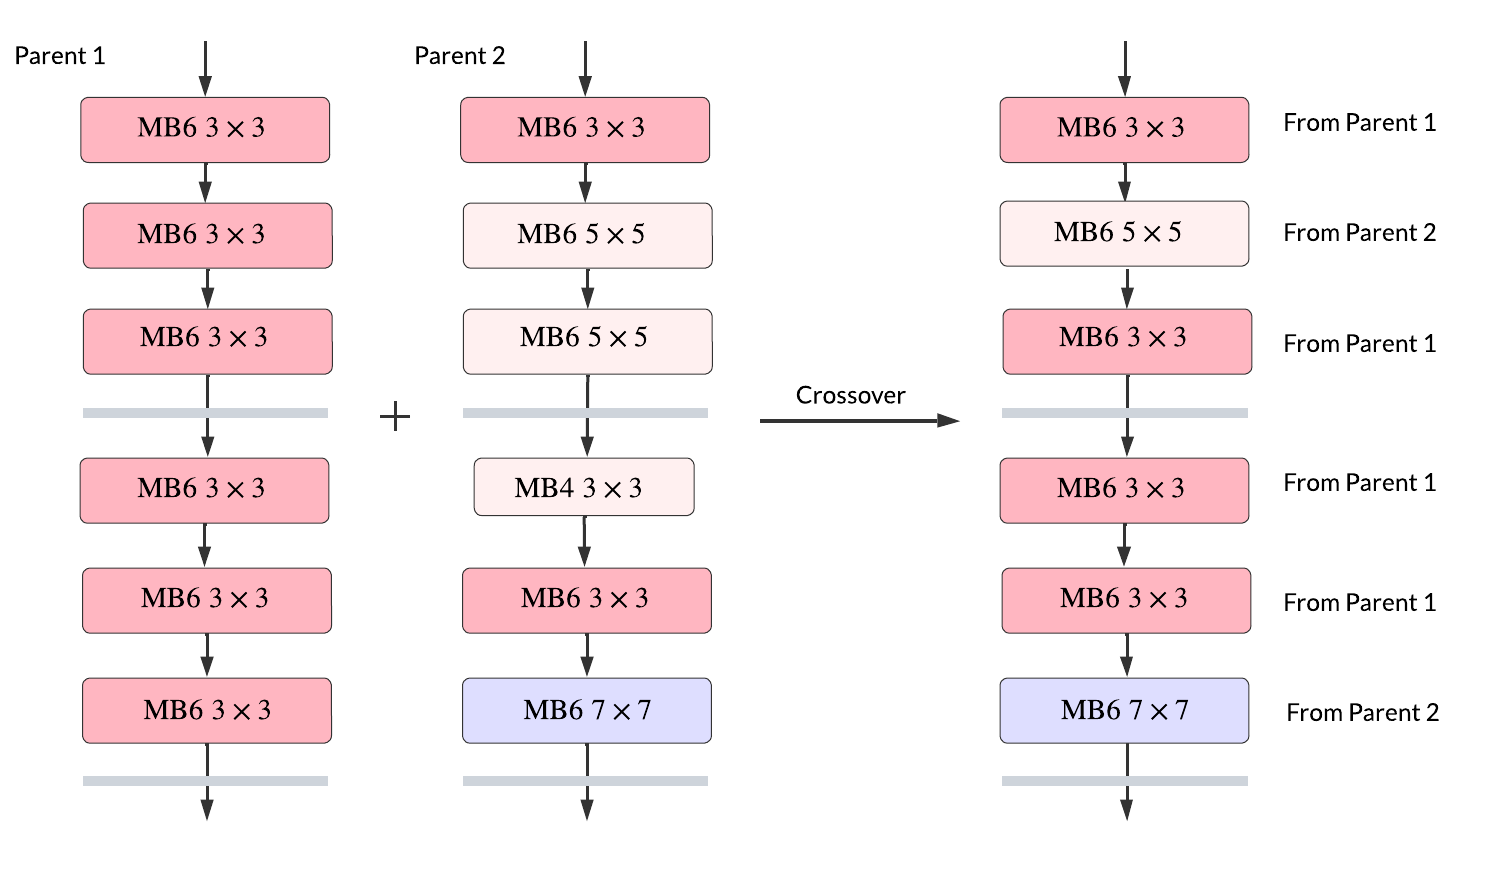
\includegraphics[width=.8\textwidth]{assets/images/crossover.png}
                        \end{center}
                        \caption{Crossover}%
                        \label{fig:hw-nas:nas:crossover}
                    \end{figure}

        \subsubsection{Bayesian Optimization}



    \subsection{Accuracy Estimation Strategy}
        The accuracy estimation strategy defines how to estimate the accuracy of a given neural network architecture in the design space. There are multiple ways in which the performance of a given neural network can be evaluated :  
    
        \subsubsection{Training from scratch}
            Training from scratch is the most naive approach. It is done by training the selected architecture from scratch on the training set and evaluating the accuracy of the trained model on the validation set.
        
            \textbf{Drawback:} it is computationally expensive and limits the number of architectures that can be explored.

        \subsubsection{Lower fidelity estimates}
            In this set of evaluation techniques, performance is estimated by measuring the accuracy after training with a reduced number of epochs~\cite{nasrl}, on a subset of the data~\cite{subset}, or on downscaled models~\cite{nasrl}, among other variations.

            \textbf{Drawback:} these methods introduce bias in the estimate as performance will typically be underestimated~\cite{NAS-survey}.
            

        \subsubsection{One-shot Evaluation}

            One-shot evaluation, often termed weight sharing, involves treating all architectures as distinct sub-networks within a larger supernetwork that is initially trained. Afterwards, the trained weights are shared among architectures that share edges in the supernetwork.~\cite{smash}
            
            \textbf{Drawback:} the predefined supernetwork restricts the search space to its sub-networks.

        \subsubsection{Zero-shot Evaluation}